\section{Virtualization}
\label{section:virtualization}

    We discovered in \autoref{subsection:provisioning} that a common scenario when provisioning infrastructure on own hardware in IIoT systems is the provisioning of virtual machines in a virtualization platform. In this section, we want to understand when this makes sense and how it is done in practice.\newline

    \begin{quote}
        ``Virtual machines have finally arrived. Dismissed for a number of years as merely academic curiosities, they are now seen as cost-effective techniques for organizing computer systems resources to provide extraordinary system flexibility and support for certain unique applications.'' -- Robert P. Goldberg, 1974 \cite{vs_anforderungsprofil}
    \end{quote}

    \noindent Virtual machines have been seen as a great opportunity from very early on. By hosting multiple virtual machines on a single physical machine, the hardware can often be used in a more efficient and flexible way. At the core of virtual machine technology is the hypervisor, often referred to as the virtual machine monitor (VMM). It is a software layer responsible for creating and running virtual machines, serving as an interface between the hardware and the virtual environments. If an operating system is installed on the machine, the hypervisor interfaces between the OS and the virtual machines. The VMM manages and virtualizes the hardware in a way that is transparent for the virtual machines. It is not differentiated between physical and virtual hardware, which means that the hardware interface provided to the operating system of the virtual machines is indistinguishable from a bare-metal server from the VM's perspective. The VMM also fully isolates virtual machines from one another in terms of resources and security, i.e.\ regarding their processing power, memory, storage or network traffic. While virtualization used to cause a loss of performance, the technology is optimized well today and hardly causes any overhead, mainly due to hardware support for virtualization like custom CPU instructions \cite{vs_anforderungsprofil}. \newline 

    \begin{figure}[htbp]
        \centering
        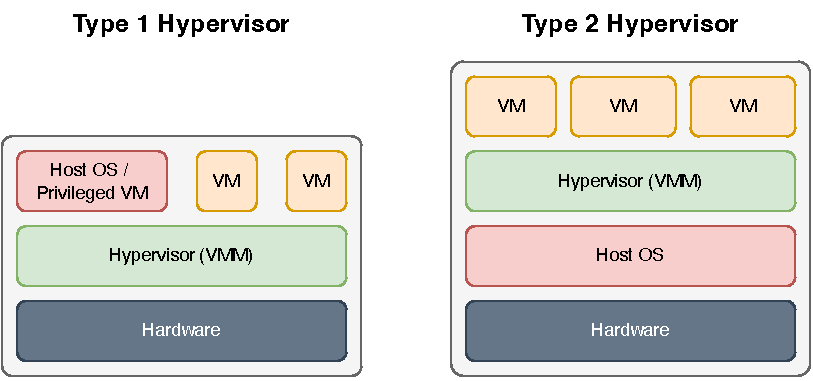
\includegraphics[width=0.7\textwidth]{img/hypervisors.pdf}
        \caption{Type 1 and Type 2 Hypervisors}
        \label{figure:hypervisors}
    \end{figure}

    \noindent Typically a distinction is made between two types of hypervisors as shown in \autoref{figure:hypervisors}. Type 1 hypervisors, also known as bare-metal hypervisors, lay directly on the hardware platform and create and run virtual machines directly on top of the hardware. This has the main benefit of offering high performance for VMs and is usually used for server systems where a high number of virtual servers is expected. In such systems, the VMs are typically centrally and remotely managed through APIs for efficient scaling capabilities. Since the hypervisor cannot rely on an underlying operating system, it has to tackle issues like managing drivers and file systems. In practice, this is often done by a trusted privileged VM that abstracts all of these challenges away for the other virtual machines. Compared to this, type 2 hypervisors which are also referred to as hosted hypervisors run on top of an operating system. This simplifies the responsibilities of the hypervisor, since the operating system already takes over the abstraction from the hardware and already has required system components like drivers. This approach however comes with the drawback of lower performance compared to type 1 hypervisors and is hence rather used for client systems, where the amount of VMs is very limited and simple UI-based management is usually enough. 
    
    When a virtualization technology is used for bare-metal machines in an IIoT platform the type 1 hypervisor should be chosen due to its high performance and API-based management, both of which allow for large-scale \cite{vs_anforderungsprofil}. \newline

    Now that we understand how virtualization works under the hood and how it should be used in an IIoT system, let us discuss why one would choose virtualization over plain bare-metal machines for provisioning (see \autoref{section:bare-metal-provisioning}). While using the hardware directly offers the best performance, using bare-metal machines still has certain drawbacks compared to a virtualized environment. Implementing multitenancy with robust isolation on bare-metal systems is challenging in contrast to simply using virtual machines, as it requires complex and often custom configurations to ensure both security and resource partitioning. This poses a problem when a single machine should be used by multiple parties that might affect each other, which could cause interference in the manufacturing/production site of an IIoT system (noisy neighbor problem). As already discovered in \autoref{section:bare-metal-provisioning} the biggest challenge however remains the lack of standardization when it comes to APIs for managing hardware directly. While there exist solutions (see \autoref{subsection:network-boot}) they are often based on outdated tools, dependent on the often very heterogeneous hardware, and are not robust due to many possible failures.\newline

    In contrast to this stands a hypervisor-based virtualized infrastructure, where each virtual machine is fully isolated from one another thus allowing for simple multipurpose usage of hardware. An example where this might be used is the deployment of a workload that cannot be containerized on a bare-metal server, which is already running Kubernetes. Using virtualization, this can easily be achieved by creating a separate isolated VM. Also, the fact that each virtual server is software-based offers enhanced infrastructure flexibility. Each server can be relocated to a different physical server effortlessly, created or destroyed on demand (``cattle not pets''), and vertically scaled by allocating more or fewer resources, among other features that expand the infrastructure's adaptability. The largest benefit however is the simple management of virtual servers through APIs. Commonly used virtualization platforms like VMware vSphere or ProxmoxVE offer rich APIs that feel similar to managing virtual machines within a cloud provider. These APIs can be used by ClusterAPI infrastructure providers directly (see \autoref{subsection:capi}) which is not only simpler but way more robust compared to the out-of-band management of bare-metal servers. Many multicluster management platforms (see \autoref{section:multicluster-mgmt}) like Rancher or Gardener that are capable of deploying Kubernetes onto a variety of infrastructure can also provision Kubernetes onto virtualization platforms directly. This way, a multicluster management solution can be used directly rather than building your own setup with ClusterAPI thus again reducing the system's complexity. 
    
    The use of virtualization on top of own hardware not only has benefits however. While with modern hardware, virtualization does not introduce much overhead anymore, the physical resources are still used a bit less efficiently due to the overhead of virtualization. Also, running a virtualization platform introduces more components and thus complexity that requires domain experts into the system. Lastly, production-ready virtualization platforms like VMware vSphere introduce additional cost, that needs to be accounted for \cite{baremetal_vs_hypervisor}. If a virtualization infrastructure already exists in the target environment however, it will simplify and robustify the provisioning mechanism immensely. \newline

    Overall, virtualization can significantly simplify the provisioning of bare-metal infrastructure for the edge and fog environments of the reference architecture described in \autoref{chapter:architecture-proposal}. Instructing ClusterAPI to interact with a virtualization platform can also improve the very crucial robustness of the infrastructure provisioning mechanism compared to using outdated out-of-band management solutions to provision hardware directly. Since drawbacks, i.e.\ cost, less efficient use of physical resources and additional complexity, exist as well, the decision whether to employ virtualization needs to be made dependent on the requirements of the project in question however.